\section{Observation Model}

Consider $p( z_i | obj)$. We will assume that $\theta_i$ is known, and thus we
just need to model $p( r_i | obj, \theta_i)$. We will do this by building a
lookup table of histograms from simulated data.

We generate a number of simulated environments with objects placed in random
positions and orientations. We then generate simulated LIDAR data from this
environment.

We take each $z_i$ generated. We project each ray into the object's frame. We
compute the relative angle between the ray and the object, $\phi = \theta_i -
\theta_{object}$. We also compute the closest distance between the ray and the
center of the object location, $d_{\text{ray}}$. Finally, we compute
$d_{\text{obs}}$, the position of the range $r_i$ along the ray, relative to the
closest point along the ray to the object center. This is depicted in
\figref{fig:obs_model}.
%
\begin{figure}
  \centering
  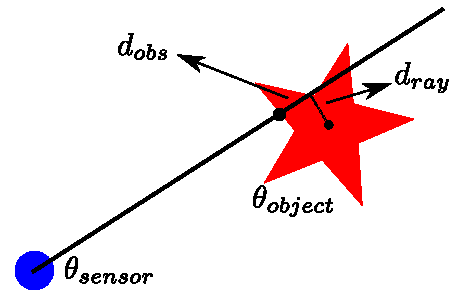
\includegraphics[width=2in]{figures/ray_model.pdf}
  \caption{Ray-based observation model for a given object. The sensor is
    depicted by the blue circle. The red star depicts the object we are
    interested in.}
  \label{fig:obs_model}
\end{figure}
%
Thus, $(\phi, d_{\text{ray}})$ parameterizes the ray for the $z_i$ that we are
considering, and $d_{\text{obs}}$ represents the observation, relative to the
object's location. (Note that these can be positive or negative). So, we have
%
\begin{align}
  p( r_i | obj, \theta_i) &=
    p_{obj}( d_{\text{obs}} | \phi, d_{\text{ray}} )
  \text{.}
\end{align}

We maintain a two-dimensional array of histograms, parameterized by $(\phi,
d_{\text{ray}})$. We discretize $\phi$ at \unit{0.05}{\rad} and
$d_{\text{ray}}$ at \unit{0.05}{\m}. For each $z_i$, we find the appropriate
histogram and update it with $d_{\text{obs}}$.

Additionally, we use negative mining in a similar fashion to estimate
$p( r_i | \lnot obj, \theta_i) = p_{\lnot obj} ( d_{\text{obs}} | \phi, d_{\text{ray}}) $.

Thus, \eqnref{eq:obj_model} becomes:
%
\begin{align}
  \log p( obj | \mathbf{Z} ) &=
   \log{\eta} + \sum_{i=1}^{n} { \log p_{obj}( d_{\text{obs}} | \phi, d_{\text{ray}}) }
   \text{,}
   \label{eq:obj_model_pos}
\end{align}
%
and we also have:
%
\begin{align}
  \log p( \lnot obj | \mathbf{Z} ) &=
   \log{\eta} + \sum_{i=1}^{n} { \log p_{\lnot obj} ( d_{\text{obs}} | \phi, d_{\text{ray}}) }
   \text{.}
   \label{eq:obj_model_neg}
\end{align}

So, by leveraging these observation models, we can compute:
%
\begin{align}
  s_{ \text{obj} }     &=
    \sum_{i=1}^{n} { \log p_{obj}( d_{\text{obs}} | \phi, d_{\text{ray}}) } \\
  s_{\lnot \text{obj}} &=
    \sum_{i=1}^{n} { \log p_{\lnot obj} ( d_{\text{obs}} | \phi, d_{\text{ray}}) } \\
  p ( obj | \mathbf{Z} ) &=
    \frac{1}{1 + \exp{(s_{\lnot \text{obj}} - s_{\text{obj}})}}
  \text{.}
  \label{eq:detection_prob}
\end{align}

To visualize our observation model and verify that it is capturing the right
thing, we can use it to generated a synthetic LIDAR scan of a object. We place
an object at $(0.0, 5.0)$ with $\theta = \unit{18}{\degree}$. For a range of
sensor angles $\theta_i$, we can evaluate $p( r_i | obj, \theta_i ) $ and thus
generate a synthetic scan that represents what we might expect to see. We depict
this in \figref{fig:synthetic_scan} evaluated at different percentiles (e.g., at
50\% we have the median observation we would expect). We do the same for
$p_{\lnot \text{obj}}$ in \figref{fig:synthetic_scan_noobj}.
%
\begin{figure}
  \centering
  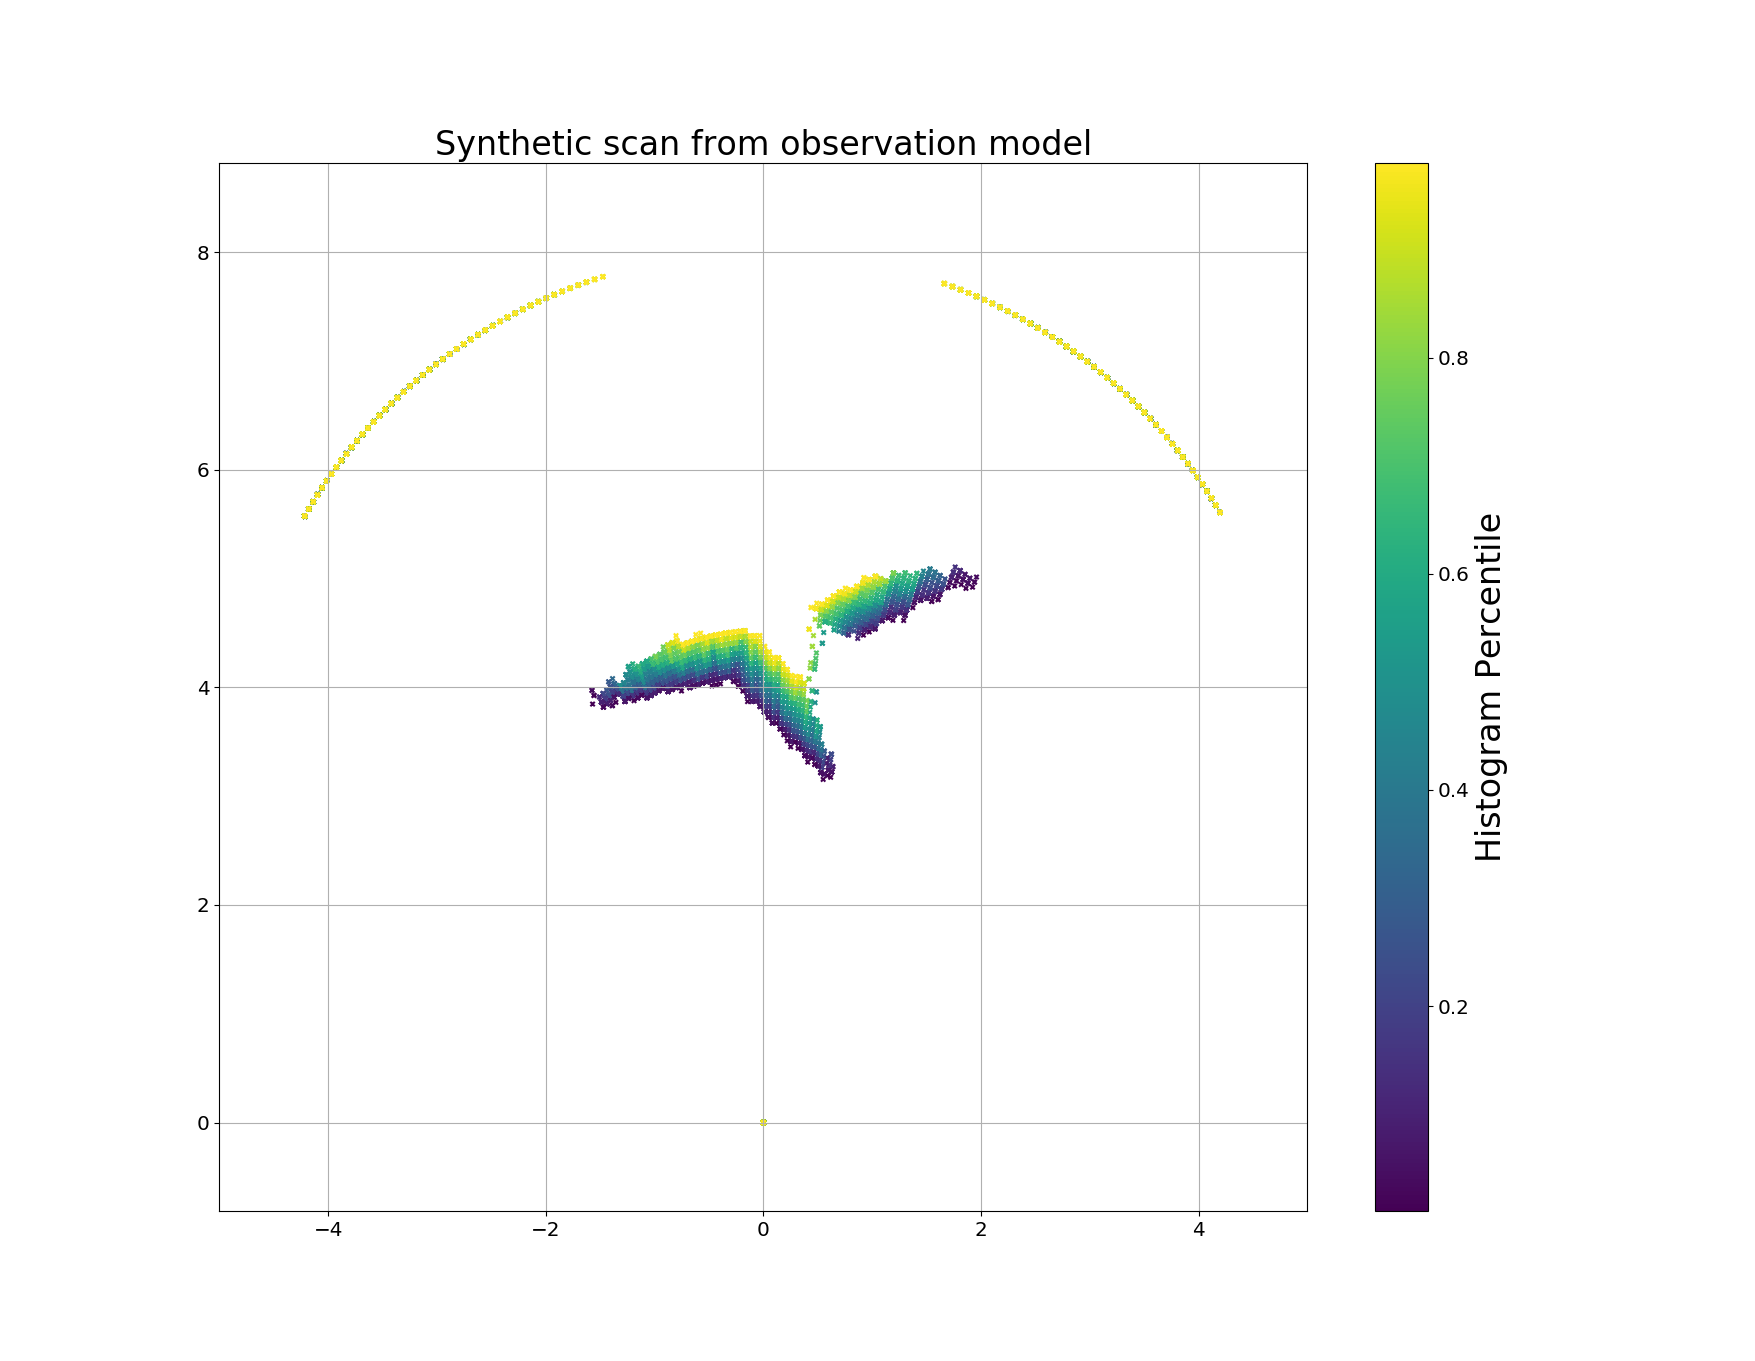
\includegraphics[width=\columnwidth]{figures/synthetic_scan.png}
  \caption{Synthetic scan created for an object at $(0.0, 5.0)$ with $\theta =
    \unit{18}{\degree}$.}
  \label{fig:synthetic_scan}
\end{figure}
%
\begin{figure}
  \centering
  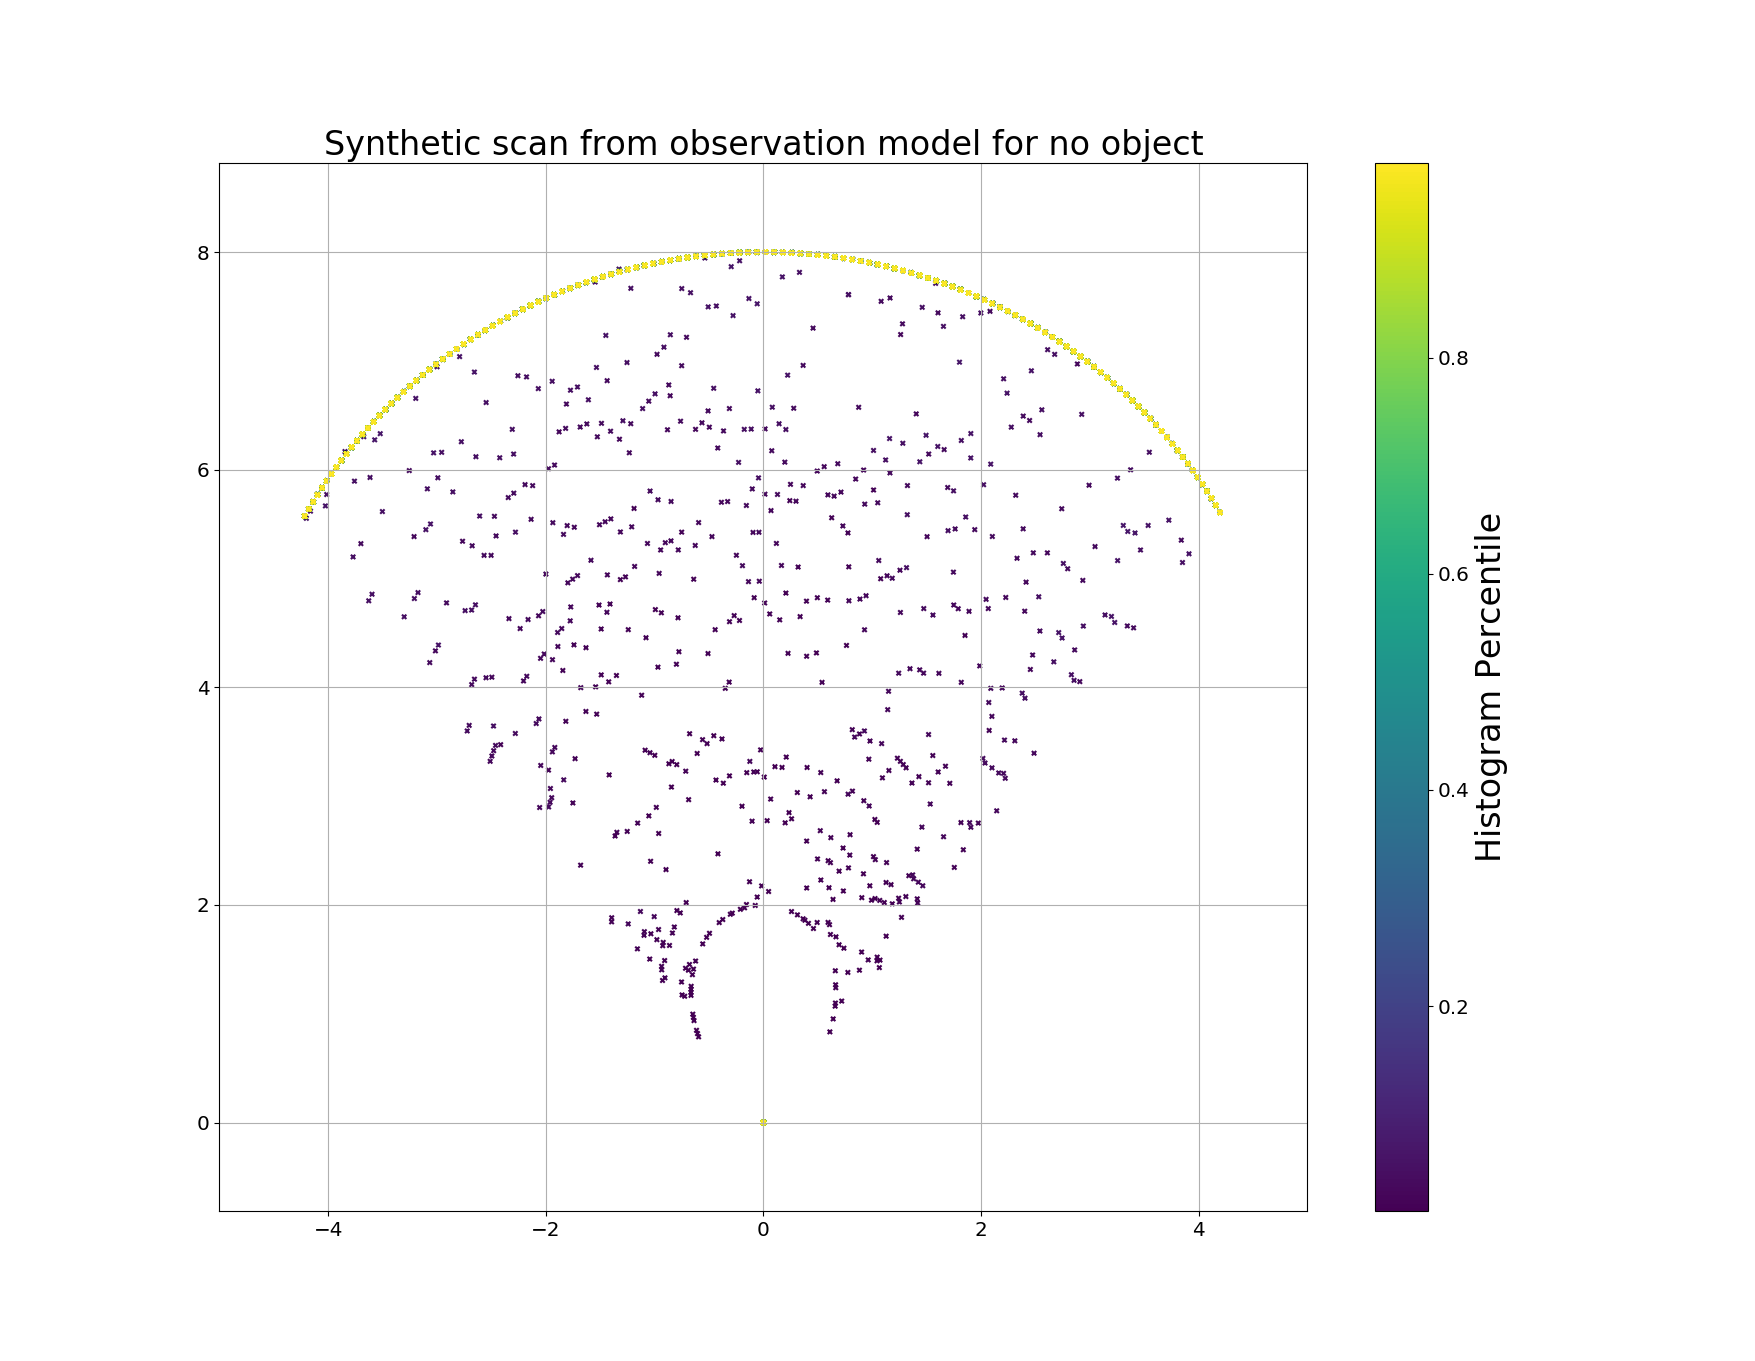
\includegraphics[width=\columnwidth]{figures/synthetic_scan_noobj.png}
  \caption{Synthetic scan created for $p_{\lnot \text{obj}}$.}
  \label{fig:synthetic_scan_nobj}
\end{figure}
